\documentclass[12pt]{amsart}

\usepackage{amsmath}
\usepackage{amssymb}
\usepackage{amsfonts}
\usepackage[alphabetic]{amsrefs}
\usepackage{amsthm}
\usepackage{enumitem}
\usepackage{fullpage}
\usepackage{graphicx}
\usepackage{caption}
\usepackage{color}
\usepackage{tikz}

\newcommand{\An}{\mathbb{A}^n}
\newcommand{\Pn}{\mathbb{P}^n}
\renewcommand{\a}{\mathfrak{a}}

\newtheorem{theorem}{Theorem}%[subsection]
\newtheorem{definition}[theorem]{Definition}
\newtheorem{corollary}[theorem]{Corollary}
\newtheorem{lemma}[theorem]{Lemma}
\newtheorem*{exercise}{Exercise}
\newtheorem{proposition}[theorem]{Proposition}

\theoremstyle{remark}
\newtheorem*{remark}{Remark}

\theoremstyle{remark}
\newtheorem*{example}{Example}

\allowdisplaybreaks

\title{Notes on Cluster Algebras}
\author{Declan Fletcher}
\date{}

\begin{document}

\maketitle

\tableofcontents

I would like to prove that the coordinate ring of a Grassmannian is a cluster algebra, perhaps starting with $\mathrm{Gr}_{2, n}$ and potentially generalising to $\mathrm{Gr}_{k, n}$.
There are a few things ingredients in being able to do this:
\begin{itemize}
	\item
	Understand the structure of $\mathrm{Gr}_{2, n}$, in particular, the Pl\"{u}cker coordinates and the coordinate ring.
	
	\item
	Understand the definition of a cluster algebra.
	
	\item
	Use these to show that the coordinate ring does have the cluster algebra structure.
\end{itemize}

\section{Affine and projective varieties}
The Grassmannian is an example of a \emph{projective variety}.
To understand what this means, we'll discuss affine varieties and their coordinate rings, before moving on to projective varieties and their coordinate rings, following the presentation in \cite[\S1.1-1.2]{Hartshorne77}.
Throughout, we will let $k$ be a fixed algebraically closed field.

\subsection{Affine varieties}
Affine $n$-space over $k$, denoted $\An_k$ or simply $\An$, is the set of $n$-tuples of elements of $k$, i.e.,
$$\An = \{(a_1, \dots, a_n) \, : \, a_i \in k\}.$$
Elements of $\An$ are called points, and if $P = (a_1, \dots, a_n)$ then the $a_i$ are called the coordinates of $P$.
Let $A = k[x_1, \dots, x_n]$ be the polynomial ring in $n$ variables over $k$, which we interpret as the ring of polynomial functions on $\An$ by defining $f(P) = f(a_1, \dots, a_n)$ for $P \in \An$ and $f \in A$.
This allows us to talk about the zeros of a polynomial $f$, namely 
$$Z(f) = \{P \in \An \, : \, f(P) = 0\}.$$
More generally, if $T$ is any set of polynomials (i.e., $T \subseteq A$), we define the zero set of $T$ as the points where all polynomials in $T$ vanish, meaning 
$$Z(T) = \{P \in \An \, : \, f(P) = 0 \text{ for all } f \in T\}.$$
Note that if $\mathfrak{a}$ is the ideal generated by $T$, then $Z(\mathfrak{a}) = Z(T)$. 
Since $A$ is a Noetherian ring (\textcolor{red}{note: prove this  --- ``Hilbert's basis theorem''}), any ideal has a finite set of generators $f_1, \dots, f_r$ and $Z(T)$ can be expressed as $Z(\{f_1, \dots, f_r\})$.

\begin{definition}
A subset $Y \subseteq \An$ is called algebraic if $Y$ is the set of common zeros of a set of polynomials, i.e., if there exists $T \subseteq A$ such that $Y = Z(T)$.
\end{definition}

\begin{example}
Any line in $\mathbb{A}^2$ is the set of zeros of the polynomial $ax + by - c$ for some $a, b, c \in k$.
Therefore lines are algebraic.
The parabola $Z(\{y - x^2\})$ is an algebraic set.
\end{example}

\begin{proposition}[{\cite[Prop 1.1]{Hartshorne77}}]
We have the following properties of algebraic sets:
\begin{enumerate}
\item
If $Y_1$ and $Y_2$ are algebraic sets , then $Y_1 \cup Y_2$ is an algebraic set.

\item
If $\{Y_i\}_{i \in I}$ is an arbitrary collection of algebraic sets, then $\bigcap_{i \in I} Y_i$ is algebraic.

\item
$\emptyset$ and $\An$ are algebraic sets.
\end{enumerate}
\end{proposition}
\begin{proof}
(1) Suppose $Y_1 = Z(T_1)$ and $Y_2 = Z(T_2)$ where $T_1, T_2 \subseteq A$.
We claim that $Y_1 \cup Y_2 = Z(T_1 T_2)$, where $T_1 T_2 = \{f g \, : \, f \in T_1, g \in T_2\}$.
If $P \in Y_1 \cup Y_2$, assume without loss of generality that $P \in Y_1$.
Then for all $f \in T_1$, $f(P) = 0$, and $(fg)(P) = 0$ for all $fg \in T_1 T_2$ so $P \in Z(T_1 T_2)$.
Let $P \in Z(T_1 T_2)$.
If $f(P) = 0$ for all $f \in T_1$, then $P \in Z(T_1) = Y_1$.
Otherwise, let $f \in T_1$ such that $f(P) \ne 0$.
Since $P \in Z(T_1 T_2)$, we have $(fg)(P) = 0$ which implies $g(P) = 0$ for all all $g \in T_2$.
This means $P \in Z(T_2) = Y_2$ and in either case $P \in Y_1 \cup Y_2$.

(2) Let $\{Y_i\}_{i \in I}$ be algebraic sets such that $Y_i = Z(T_i)$ for each $i$.
Then
$$\bigcap_{i \in I} Y_i = \bigcap_{i \in I} Z(T_i) = \{P \in \An \, : \, f(P) = 0 \text{ for all } f  \in T_i, \text{ for all } i \in I\} = Z\left( \bigcup_{i \in I} T_i\right).$$

(3) Note that $\emptyset = Z(\{1\})$ and $\An = Z(\{0\})$.
\end{proof}

\begin{example}
The lines $y - x = 0$ and $y + x = 0$ are algebraic, and their union is defined by $y^2 - x^2 = (y-x)(y+x) = 0$.
If $\{Y_a\}_{a \in k}$, where each $Y_a = Z(\{y=ax\})$, is the set of lines through the origin, then $\bigcap Y_a = Z \left(\bigcup Y_a\right) = \{(0, 0)\}$.
Therefore $\{(0, 0)\}$ is an algebraic set in $\mathbb{A}^2$. 
\end{example}

\begin{definition}[Zariski topology]
The Zariski topology is on $\An$ is defined by taking the open subsets to be the complements of the algebraic sets, i.e., the algebraic sets are the closed sets.
The previous proposition implies this satisfies the axioms for a topology.
\end{definition}

\begin{example}[The Zariski topology on $\mathbb{A}^1$]
Let $Z(T)$ be an algebraic set where $T \subseteq A = k[x]$.
Since $Z(T) = Z(\mathfrak{a})$ for $\mathfrak{a} = \langle T \rangle$, and every ideal in $k[x]$ is principal (\textcolor{red}{note: prove this}), $Z(T) = Z(\{f\})$ for some $f \in A$.
So every algebraic set in $\mathbb{A}^1$ is the zero set of a single polynomial.
Further, since $k$ is algebraic closed, any nonconstant $f$ can be written $f = c(x - a_1) \dots (x-a_n)$ for some $c, a_i \in k$.
So $Z(T) = Z(\{f\}) = \{a_1, \ldots, a_n\}$, meaning we can conclude every algebraic set in $\mathbb{A}^1$ is simply a finite set of points (or $\emptyset$ or $\mathbb{A}^1$).
Correspondingly, the open sets are $\emptyset$, $\mathbb{A}^1$, and the complements of finite sets.
Note this implies the Zariski topology is not Hausdorff;
if we try to find open sets $U$ and $V$ that separate the points, say, $0$ and $1$, $U$ and $V$ will contain an infinite number of points and must necessarily intersect.
\end{example}

\begin{definition}[Irreducible set]
A nonempty subset $Y$ of a topological space $X$ is irreducible if it cannot be expressed as the union $Y = Y_1 \cup Y_2$ of two proper subsets which are each closed in $Y$.
The empty set is not considered to be irreducible.
\end{definition}

\begin{example}
$\mathbb{A}^1$ is irreducible because its only proper subsets are finite yet it is infinite ($k$ is necessarily infinite since it is algebraically closed).
The algebraic set $Z(y^2 - x^2)$ is reducible since $Z(y^2 - x^2) = Z(y - x) \cup Z(y +x)$.
\end{example}

\begin{definition}[Affine algebraic variety]
An affine algebraic variety (or simply affine variety) is an irreducible closed subset on $\An$ with the induced topology.
An open subset of an affine variety is a quasi-affine variety.
\end{definition}

Affine and quasi-affine varieties are the first objects of study in algebraic geometry.
However, the study of these objects rely deeply on the relationship between subsets of $\An$ and ideals in $A$, so we need to investigate this relationship further (this will help us give examples of affine varieties).
For a subset $Y \subseteq \An$, define the ideal of $Y$ in $A$ by
$$I(Y) = \{f \in A \, : \, f(P) = 0 \text{ for all } P \in Y\}.$$
Now we have the function $Z$ which maps subsets of $A$ to algebraic sets, and $I$ which maps subsets of $\An$ to ideals.

Establishing the connection between ideals and sets relies on Hilbert's famous \emph{Nullstellensatz}:

\begin{theorem}[Hilbert's Nullstellensatz]
Let $k$ be an algebraically closed field, let $\a$ be an ideal in $A = k[x_1, \dots, x_n]$, and let $f \in A$ be a polynomial which vanishes at all points of $Z(\a)$.
Then $f^r \in \a$ for some integer $r > 0$.
\end{theorem}

This implies the following:

\begin{proposition}[{\cite[Prop 1.2]{Hartshorne77}}]
We have the following propeties of $Z$ and $I$:
\begin{enumerate}[label=(\roman*)]
\item
If $T_1 \subseteq T_2$ are subsets of $A$, then $Z(T_1) \supseteq Z(T_2)$.

\item
If $Y_1 \subseteq Y_2$ are subsets of $\An$, then $I(Y_1) \supseteq I(Y_2)$.

\item
For any two subsets $Y_1, Y_2 \subseteq \An$, we have $I(Y_1 \cup Y_2) = I(Y_1) \cap I(Y_2)$.

\item
For any ideal $\a \subseteq A$, $I(Z(\a)) = \sqrt{\a}$, the radical of $\a$.

\item
For any subset $Y \subseteq \An$, $Z(I(Y)) = \bar Y$, the (Zariski) closure of $Y$.
\end{enumerate}
\end{proposition}
\begin{proof}
(i) If all polynomials in $T_2$ vanish at $P$, then in particular all polynomials in $T_1$ vanish at $P$.

(ii) If $f$ is polynomial which vanishes at all $P \in Y_2$, then in particular $f$ vanishes at all $P \in Y_1$.

(iii) \textcolor{red}{complete this}.
\end{proof}

\begin{corollary}[{\cite[Coro 1.4]{Hartshorne77}}]
There is a one-to-one inclusion-reversing correspondence between algebraic sets in $\An$ and radical ideals (i.e., ideals which are equal to their own radical) in $A$, given by $Y \mapsto I(Y)$ and $\a \mapsto Z(\a)$.
Furthermore, an algebraic set is irreducible if and only if its ideal is prime.
\end{corollary}
\begin{proof}
The first sentence is a direct consequence of (i), (ii), (iv) and (v) in the previous proposition.
Suppose $Y$ is irreducible.

\end{proof}

\begin{example}
This allows us to see $y = x^2$ is irreducible.
\end{example}

\begin{definition}[Affine coordinate ring]
If $Y \subseteq \An$ is an affine algebraic set, we define the affine coordinate ring of $Y$, denoted $A(Y)$, to be $A/I(Y)$.
\end{definition}

\begin{example}
The condition that an algebraic variety be irreducible implies $A(Y)$ is an integral domain.
\textcolor{red}{Do an example and a counter-example}.
\end{example}

\begin{example}
Coordinate ring of a line is $k[x]$.
\end{example}

\subsection{Projective varieties}
Projective varieties are similar to affine varieties, but are instead subsets of \emph{projective space}.
Projective space is the set of lines in an affine space.
Formally, projective $n$-space over $k$, denoted $\Pn_k$ or $\Pn$, is
$$\Pn = \{(a_0, \ldots, a_n) \ne (0, \ldots, 0) \, : \, a_i \in k \} / \sim$$
where
$$(a_0, \ldots, a_n) \sim (\lambda a_0, \ldots, \lambda a_n)$$
for all $\lambda \in k \setminus \{0\}$.
In other words, $\Pn$ is $\mathbb{A}^{n+1} \setminus \{(0, \ldots, 0)\}$ where lines lying on the same line through the origin are identified.

\textcolor{red}{
Question: why do we define projective space this way/why are we interested in this space?
Projective space has the property that any two lines intersect in a point, which is a nice property that fails in affine space when lines are parallel.
Let's consider the specific case of $\mathbb{RP}^2$.
The set of points with nonzero $z$ coordinate all have an equivalence class rep of the form $(x : y : 1)$ where there are no longer any restrictions on $x$ and $y$.
So there is a copy of $\mathbb{R}^2$ inside $\mathbb{RP}^2$.
Lines in $\mathbb{RP}^2$ correspond to planes through the origin in $\mathbb{R}^3$ so consider the planes (in $\mathbb{R}^3$) with equations $x = 0$ and $z - x = 0$. 
If we``project" onto $(x : y : 1)$, these lines look like $x = 0$ and $x = 1$, which don't intersect.
However, in $\mathbb{RP}^2$ the lines intersect at the point $(0 : 1 : 0)$ which is somehow a ``point at infinity". 
My problem is that we could equally look at the copy of $\mathbb{R}^2$ inside $\mathbb{RP}^2$ with all points of the form $(x : 1 : z)$, where the projection of the lines in $\mathbb{RP}^2$ are no longer parallel (they just look like $x = 0$ and $z = x$ with an intersection at the origin). 
How do we reconcile these different views of $\mathbb{RP}^2$ intuitively, and how should we think of $\mathbb{R}^2$ living in $\mathbb{RP}^2$ with points at infinity when there are multiple copies of $\mathbb{R}^2$ in this way?
Generally, why are projective spaces important?
}

\section{The Grassmannian as a projective variety}



\section{Cluster Algebras defined by quivers}
Unlike ``most'' commutative rings, a cluster algebra is not directly defined by generators and relations.
Instead, cluster algebras are defined as a certain subring of an ambient field $\mathcal{F}$ of rational functions in $n$ variables.
Using initial data called a \emph{seed}, which contains generators called \emph{cluster variables} and the \emph{exchange matrix}, an iterative procedure called \emph{mutation} produces the rest of the cluster variables (where how the variables mutate is based on the entries in the exchange matrix).
The cluster algebra is then defined to the subring of $\mathcal{F}$ generated by all the cluster variables.

Instead of immediately defining a cluster algebra with an exchange matrix, we'll start with an easy definition, namely a cluster algebra defined by a quiver.
This definition is a specific case of the more general definition, though is easier to visualise through the use of quivers.
Before we can define cluster algebras from quivers, we need to discuss \emph{quiver mutation}.
Our definitions in this section come from \cite[\S 2.1]{Williams14}.

\begin{definition}[Quiver]
A quiver $Q$ is an oriented graph given by a set of vertices $Q_0$, a set of arrows $Q_1$, and two maps $s : Q_1 \to Q_0$ and $t : Q_1 \to Q_0$ taking an arrow to its source and target, respectively.
\end{definition}

A quiver is finite if there are a finite number of vertices and arrows.
A loop is an arrow where the source and target are the same.
A 2-cycle is a pair of distinct arrows $\beta$ and $\gamma$ such that $s(\beta) = t(\gamma)$ and $t(\beta) = s(\gamma)$.
In the context of defining cluster algebras, we assume the quivers we work with have \emph{no loops and no 2-cycles}.

\begin{definition}[Quiver mutation]
Let $Q$ be a quiver and $k$ a vertex in $Q$.
The mutated quiver $\mu_k(Q)$ is defined as having the same vertices as $Q$, and its arrows are obtained by the following procedure:
\begin{enumerate}
\item
For each subquiver $i \to k \to j$, add a new arrow $i \to j$;

\item
Reverse all arrows with source or target $k$;

\item
Repeatedly remove 2-cycles until unable to do so.
\end{enumerate}
\end{definition}

\begin{example}
The following shows an example of quiver mutation with steps:

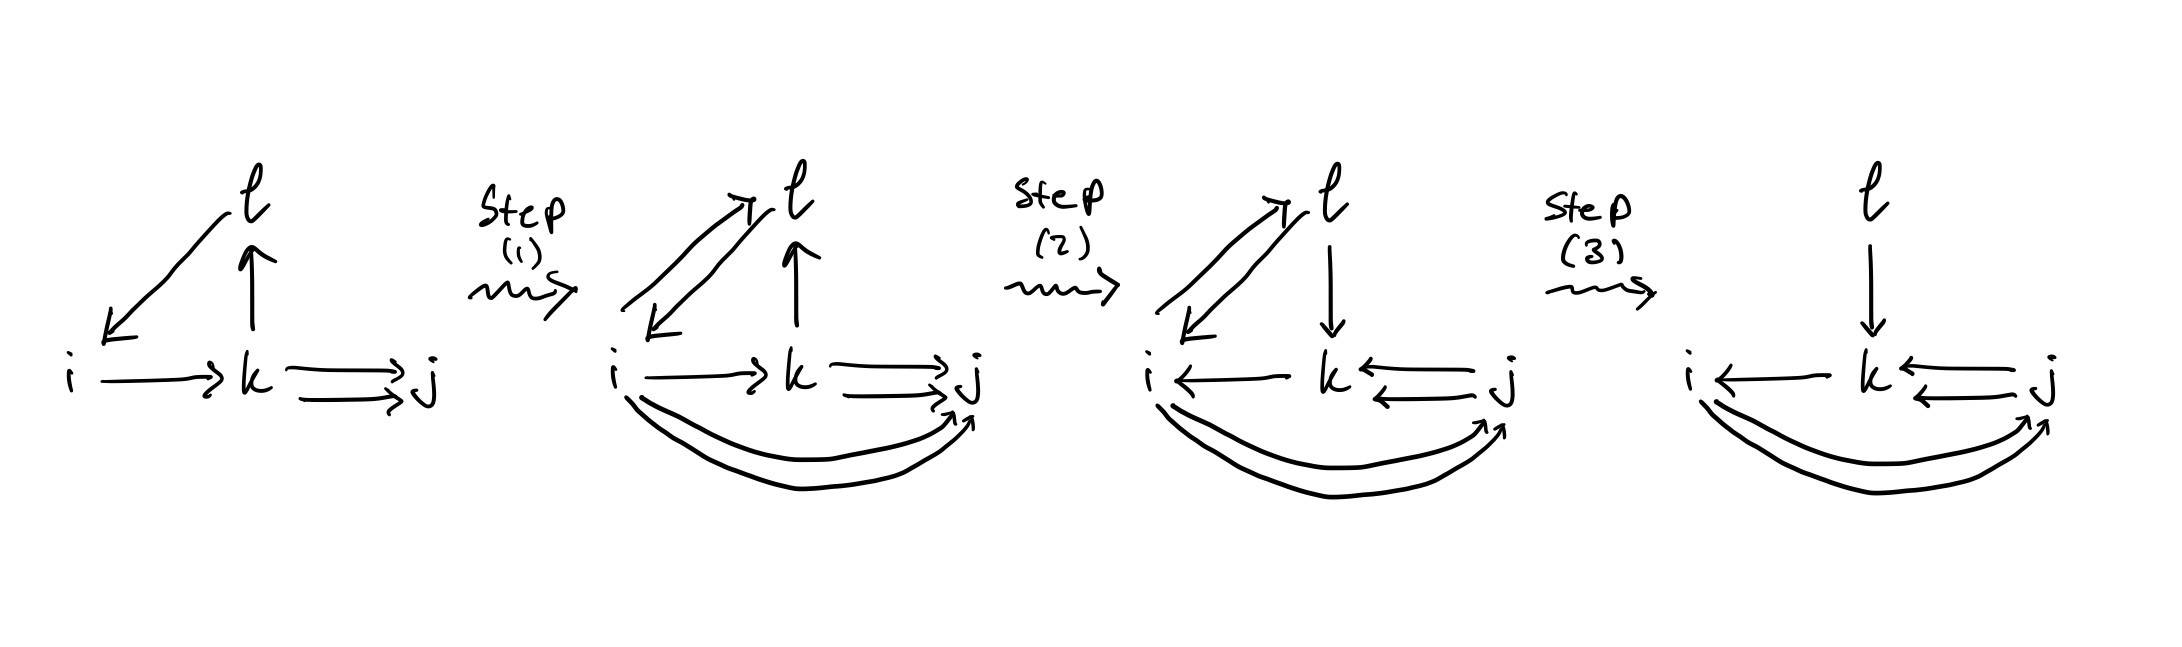
\includegraphics[width=\textwidth]{quiver_mutation}

\end{example}

\begin{remark}
Note that quiver mutation is an involution, i.e., $\mu_k(\mu_k(Q)) = Q$.
\textcolor{red}{Explain why}.
\end{remark}

\begin{definition}[Labeled seed]
Choose positve integers $m$ and $n$ with $m \ge n$.
Let $\mathcal{F}$ be an \emph{ambient field} of rational functions in $n$ independent variables over $\mathbb{Q}(x_{n+1}, \ldots, x_m)$.
A labelled seed in $\mathcal{F}$ is a pair $(\bold x, Q)$, where
\begin{itemize}
\item
$\bold x = (x_1, \ldots, x_m)$ is a free generating set for $\mathcal{F}$, and

\item
$Q$ is a quiver on vertices $1, 2, \ldots, n, n+1, \ldots, m$ whose vertices $1, 2, \ldots, n$ are called \emph{mutable} and whose vertices $n+1, \ldots, m$ are called \emph{frozen}.
\end{itemize}
We refer to $\bold x$ as the (labeled) \emph{extended cluster} of a labeled seed $(\bold x, Q)$.
The variables $\{x_1, \ldots, x_n\}$ are called \emph{cluster variables}, and the variables $c = \{x_{n+1}, \ldots, x_m\}$ are called \emph{frozen} or \emph{coefficient variables}.
\end{definition}

\begin{definition}[Seed mutation]
Let $(\bold x, Q)$ be a labeled seed in $\mathcal{F}$, and let $k \in \{1, \ldots, n\}$.
The \emph{seed mutation} $\mu_k$ in direction $k$ transforms $(\bold x, Q)$ into the labeled seed $\mu_k(\bold x, Q) = (\bold x', \mu_k(Q))$, where the cluster $\bold x' = (x_1', \ldots, x_m')$ is defined as follows:
$x_j' = x_j$ for $j \ne k$ and $x_k' \in \mathcal{F}$ is determined by the \emph{exchange relation}
$$x_k x_k' = \prod_{\substack{\alpha \in Q_1 \\ s(\alpha) = k}} x_{t(\alpha)} + \prod_{\substack{\alpha \in Q_1 \\ t(\alpha) = k}} x_{s(\alpha)},$$
where the empty product is $1$ by convention.
\end{definition}

\begin{remark}
Note that arrows between frozen vertices do not affect seed mutation as they don't affect the mutated quiver or the exchange relation.
Therefore, we can omit arrows between frozen vertices.
\end{remark}

\begin{definition}[Patterns]
Consider the $n$-regular tree $\mathbb{T}_n$ whose edges are labeled by the numbers $1, \ldots, n$, so that the $n$ edges emanating from each vertex receive different labels.
A \emph{cluster pattern} is an assignment of a labeled seed $\Sigma_t = (\bold x_t, Q_t)$ to every vertex $t \in \mathbb{T}_n$, such that the seeds assigned to the end-points of any edge $t \,\, \overset{k}{\mbox{\----}} \,\, t'$ are obtained from each other by the seed mutation in direction $k$.
The components of $\bold x_t$ are written as $\bold x_t = (x_{1;t}, \ldots, x_{n;t})$.
\end{definition}

Since any labeled seed in a pattern can reach any other by a sequence of mutations, a cluster pattern is uniquely determined by an arbitrary seed.

\begin{definition}[Cluster algebra]
Given a cluster pattern, we denote
$$\mathcal{X} = \bigcup_{t \in \mathbb{T}_n} \bold x_t = \{x_{i, t} \, : \, t \in \mathbb{T}_n, 1 \le i \le n\},$$
the set of all cluster variables in all seeds in the pattern.
The cluster algebra $\mathcal{A}$ associated with a given pattern is the $\mathbb{Z}[c]$-subalgebra of the ambient field $\mathcal{F}$ generated by all the cluster variables, i.e., $\mathcal{A} = \mathbb{Z}[c][\mathcal{X}]$.
We denote $\mathcal{A} = \mathcal{A}(\bold x, Q)$, where $(\bold x, Q)$ is any seed in the underlying cluster pattern.
In this generality, $\mathcal{A}$ is called a cluster algebra from a quiver.
We say $\mathcal{A}$ has \emph{rank} $n$ as each cluster contains $n$ cluster variables.
\end{definition}

\begin{example}
We now give a detailed example to demonstrate labeled seeds, seed mutation and patterns, and the corresponding cluster algebra.
The starting labeled seed will be $\Sigma_0 = (\{x_1, x_2\}, Q_0)$, where $Q_0$ is the quiver 

\centerline{
\includegraphics[width=0.4\textwidth]{simple_quiver}}

\noindent
with no frozen vertices for simplicity.
We can only mutate in direction $1$ or $2$, so the pattern formed is the line

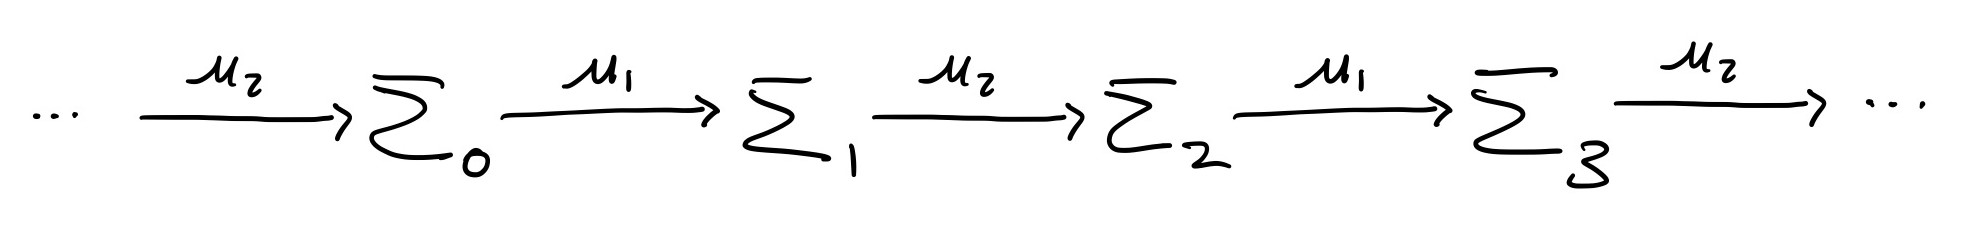
\includegraphics[width=0.9\textwidth]{simple_pattern}

\noindent
A priori, this pattern is infinite, though we will see that the sequence of labeled seeds is periodic and the pattern can be considered to form a closed finite loop.

We first mutate in direction $1$.
The new labeled seed is $\{x_1', x_2'\} = \{x_1', x_2\}$, where
$$x_1 x_1' = \prod_{\substack{\alpha \in Q_0 \\ s(\alpha) = k}} x_{t(\alpha)} + \prod_{\substack{\alpha \in Q_0 \\ t(\alpha) = k}} x_{s(\alpha)} = x_2 + 1 
\implies x_1' = \frac{x_2 + 1}{x_1} =: x_3.$$
Note the quiver mutation simply flips the direction of the arrow in $Q_0$.
So after mutating in direction $1$, the labeled seed is $\Sigma_1 = \mu_1(\{x_1, x_2\}, Q_0) = (\{x_2, x_3\}, Q_1 = x_3 \leftarrow x_2)$.

Now we mutate in direction $2$.
The new cluster variable will satistfy
$$x_2 x_2' = \prod_{\substack{\alpha \in Q_1 \\ s(\alpha) = k}} x_{t(\alpha)} + \prod_{\substack{\alpha \in Q_1 \\ t(\alpha) = k}} x_{s(\alpha)} = x_3 + 1
\implies x_2' = \frac{x_3 + 1}{x_2} = \frac{x_1 + x_2 + 1}{x_1 x_2} =: x_4.$$
So we get $\Sigma_2 = (\{x_3, x_4\}, Q_2 = x_3 \to x_4\})$.

Next we mutate in direction $1$.
The exchange relation is
$$x_3 x_3' =  \prod_{\substack{\alpha \in Q_2 \\ s(\alpha) = k}} x_{t(\alpha)} + \prod_{\substack{\alpha \in Q_2 \\ t(\alpha) = k}} x_{s(\alpha)} = x_4 + 1 
\implies x_3' = \frac{x_4 + 1}{x_3} = \frac{x_1 + 1}{x_2} =: x_5.$$
So we get $\Sigma_3 = (\{x_4, x_5\}, Q_3 = x_5 \leftarrow x_4)$.

Next we mutate in direction $2$.
The exchange relation is 
$$ 
x_4 x_4' =  \prod_{\substack{\alpha \in Q_3 \\ s(\alpha) = k}} x_{t(\alpha)} + \prod_{\substack{\alpha \in Q_3 \\ t(\alpha) = k}} x_{s(\alpha)} = x_5 + 1
\implies x_4' = \frac{x_5 + 1}{x_4} = x_1.
$$
So then $\Sigma_4 = (\{x_1, x_5\}, Q_4 = x_5 \to x_1)$.

Now we mutate in direction $1$.
The exchange relation is
$$ 
x_5 x_5' =  \prod_{\substack{\alpha \in Q_4 \\ s(\alpha) = k}} x_{t(\alpha)} + \prod_{\substack{\alpha \in Q_4 \\ t(\alpha) = k}} x_{s(\alpha)} = x_1 + 1
\implies x_5' = \frac{x_1 + 1}{x_5} = x_2.
$$
So we get $\Sigma_5 = (\{x_1, x_2\}, Q_5 = x_2 \leftarrow x_1)$.
Note that $\Sigma_5 = \Sigma_0$ since the cluster variables are the same and the quivers are the same up to a relabelling of the vertices!

This implies that the seed pattern forms a pentagon as so:

\centerline{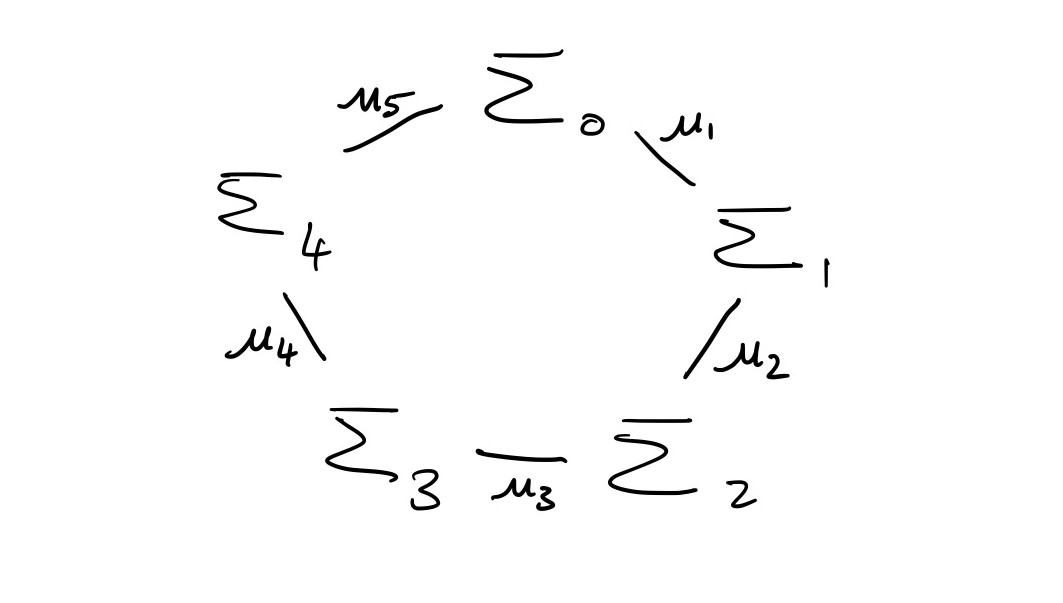
\includegraphics[width=0.7\textwidth]{closed_pattern}}

The complete set of cluster variables is
$$\mathcal{X} = \left\{x_1, x_2, x_3 = \frac{x_2 + 1}{x_1}, x_4 = \frac{x_1 + x_2 + 1}{x_1 x_2}, x_5 \frac{x_1 + 1}{x_2}\right\},$$
and the cluster algebra is
$$\mathcal{A} = \mathcal{A}(\{x_1, x_2\}, Q_0) = \mathbb{Z}\left[x_1, x_2, x_3, x_4, x_5\right].$$
\end{example}

\begin{example}
For another example, consider the initial seed
$$\Sigma_0 = (\{x_1, x_2, x_3\}, Q_0 = 1 \to 2 \to 3).$$
By definition, the seed pattern is the $3$-regular tree

\centerline{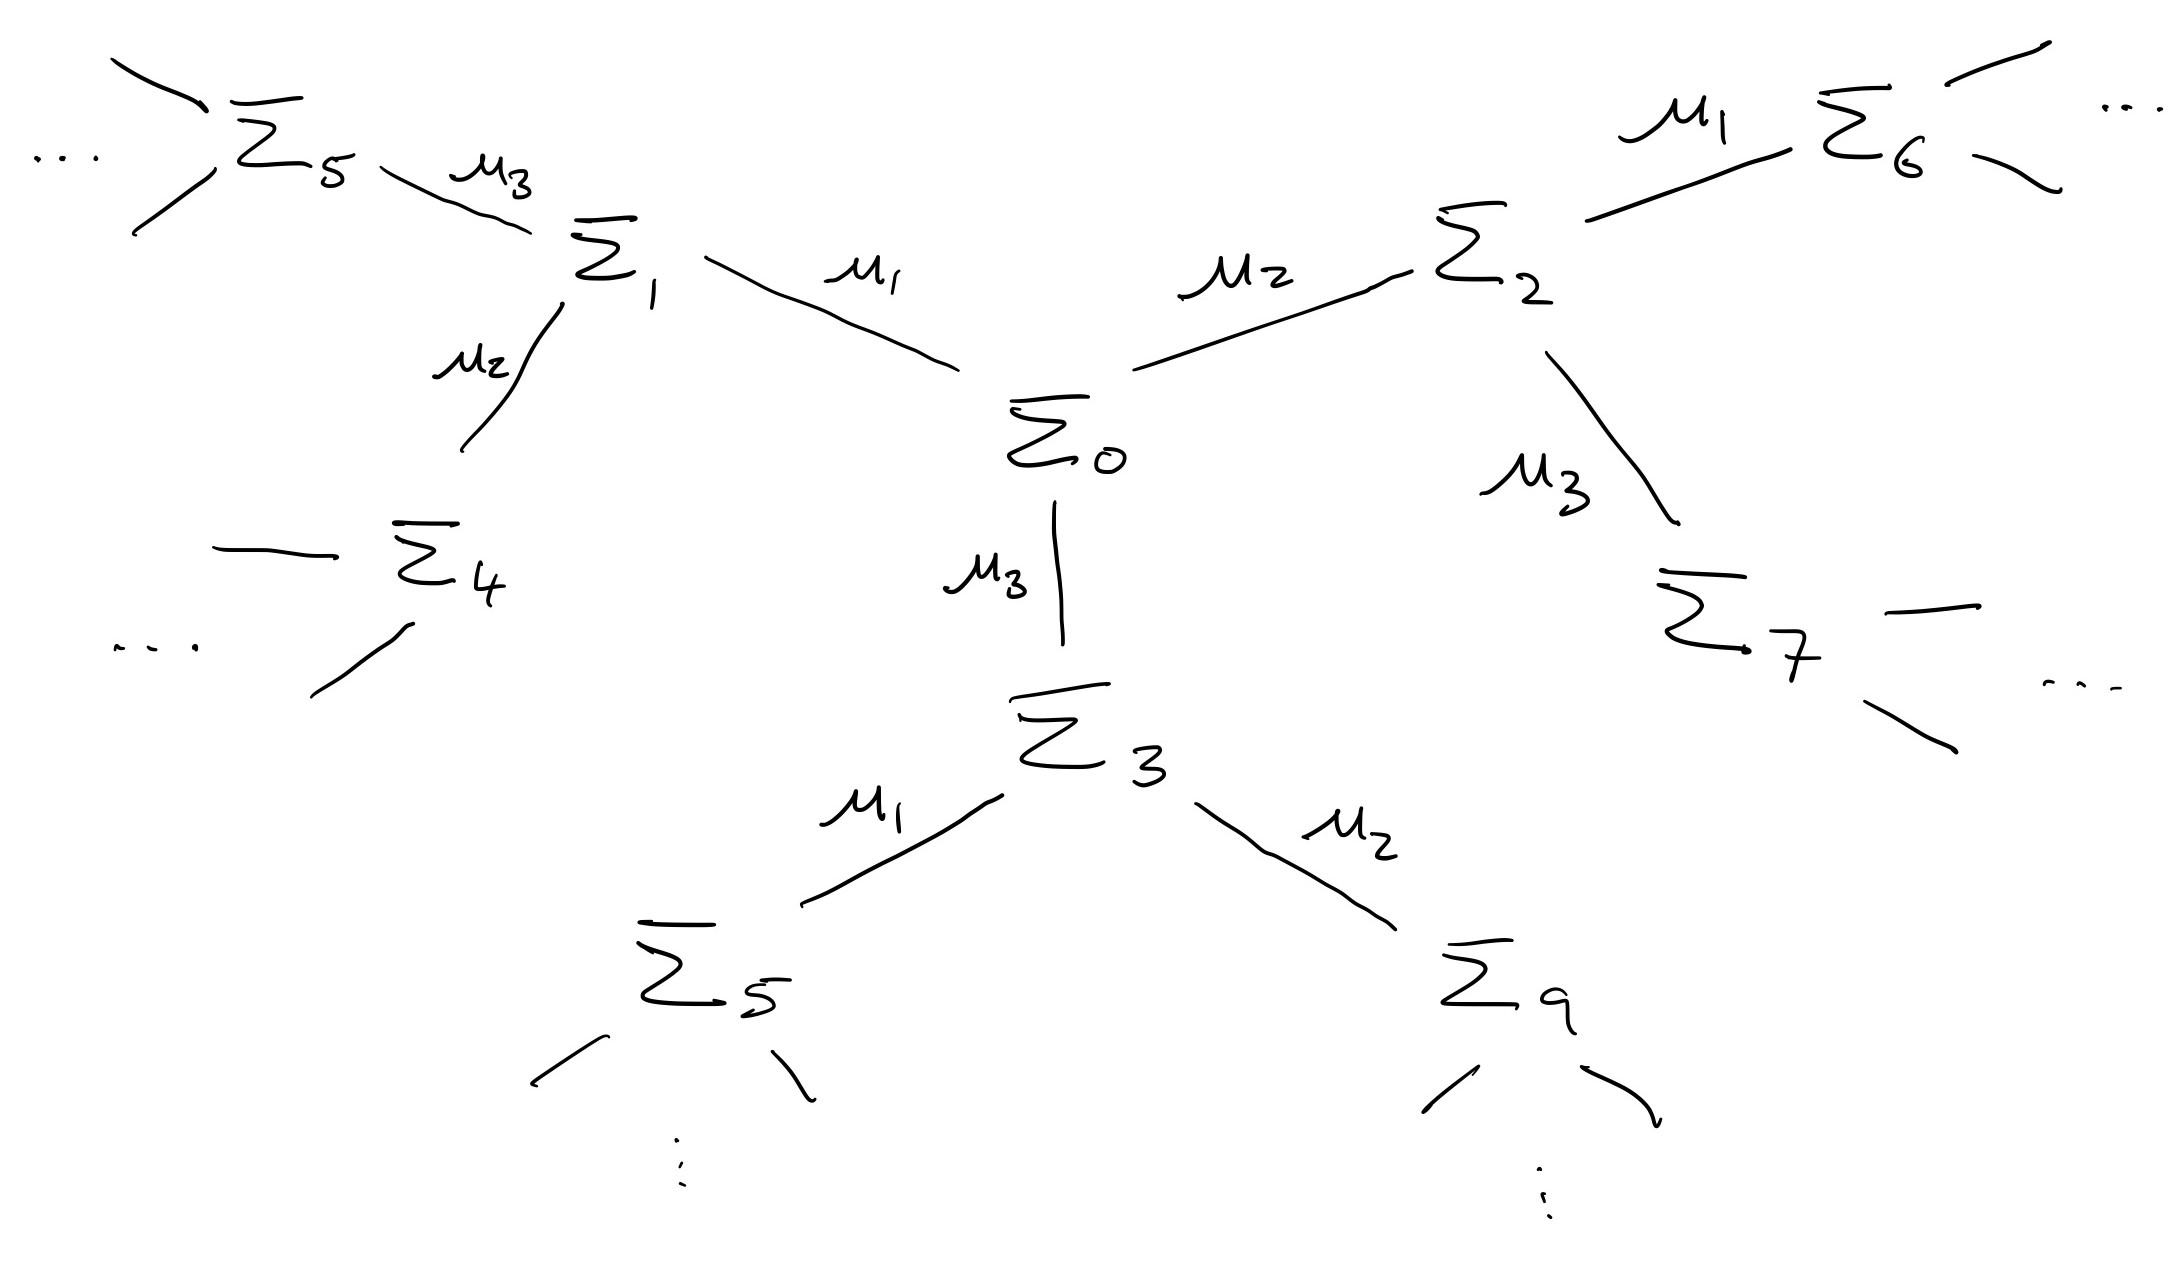
\includegraphics[width=\textwidth]{seed_pattern_2}}

\noindent
but again, the seed pattern closes up and there are a finite number of labeled seeds and hence cluster variables!
The seed pattern forms the $1$-skeleton of a polytope called the \emph{associahedron}:

\centerline{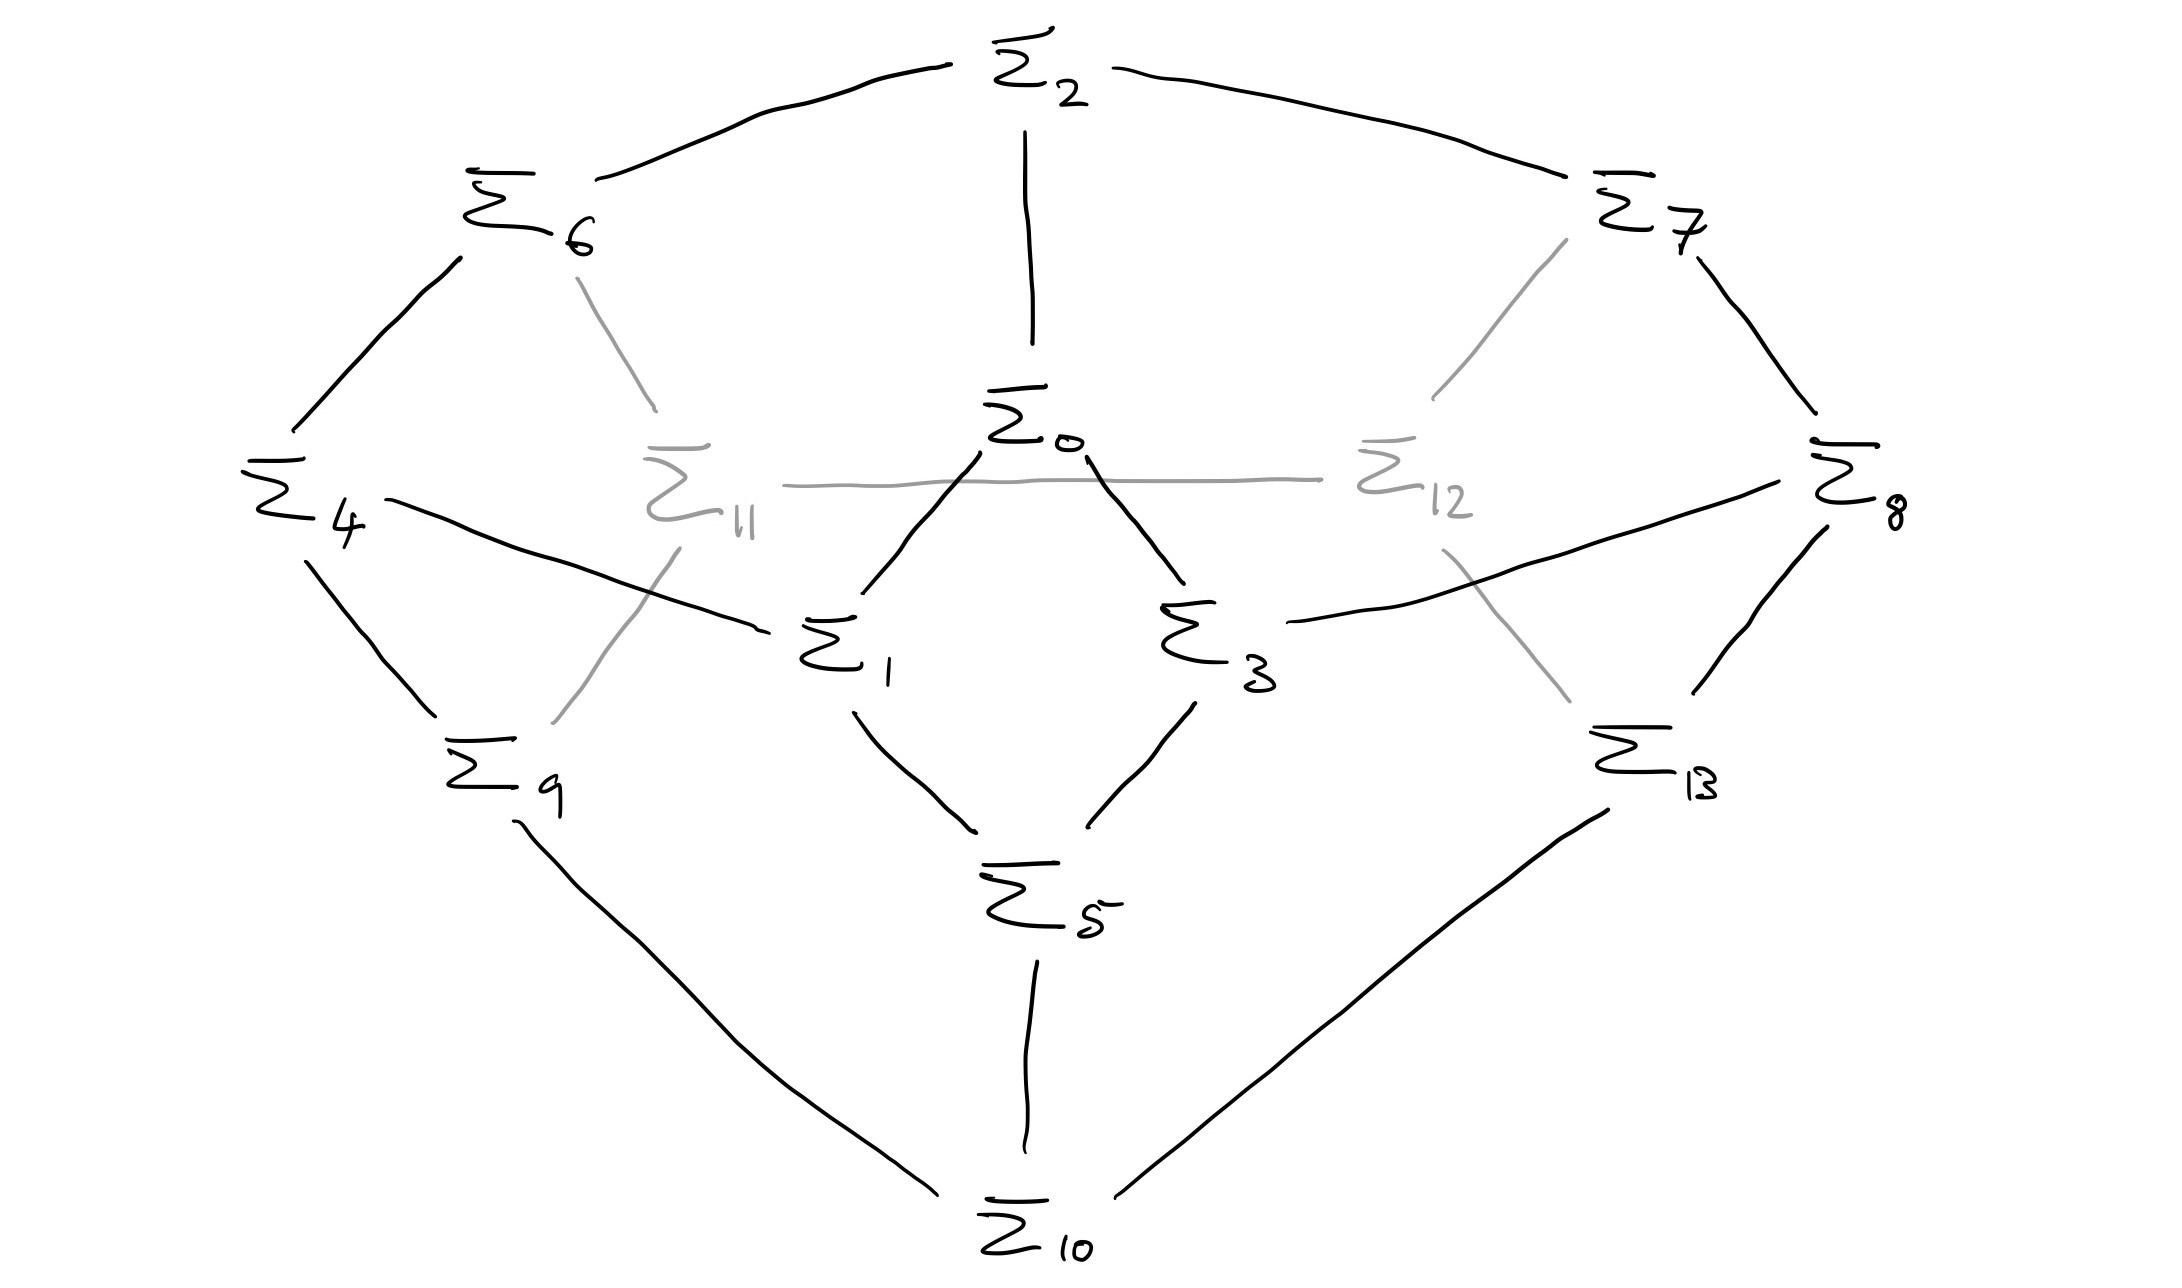
\includegraphics[width=\textwidth]{associahedron}}

\noindent
\textcolor{red}{(To do: add $\mu_i$'s to edges. Also add a list of cluster variables and quivers.)}
\end{example}

Note that these two examples given are cluster algebras of \emph{finite type}, meaning there are finitely many seeds.
In \cite{FS03}, Fomin and Zelevinsky classify finite type cluster algebras.
Remarkably, the classification is parallel to the Cartan-Killing classification of complex semisimple Lie algebras, and in particular, the finite type cluster algebras are also classified by Dynkin diagrams.
The two examples above are the cluster algebras of type $A_2$ and $A_3$.
\textcolor{red}{Add more on how to get a cluster algebra from a Dynkin diagram to explain why these are type $A_2$, $A_3$.)}
 
\begin{bibdiv}
\begin{biblist}
\bib{FS03}{article}{
   author={Fomin, Sergey},
   author={Zelevinsky, Andrei},
   title={Cluster algebras. II. Finite type classification},
   journal={Invent. Math.},
   volume={154},
   date={2003},
   number={1},
   pages={63--121},
   issn={0020-9910},
   review={\MR{2004457}},
   doi={10.1007/s00222-003-0302-y},
}

\bib{Hartshorne77}{book}{
   author={Hartshorne, Robin},
   title={Algebraic geometry},
   series={Graduate Texts in Mathematics},
   volume={No. 52},
   publisher={Springer-Verlag, New York-Heidelberg},
   date={1977},
   pages={xvi+496},
   isbn={0-387-90244-9},
   review={\MR{0463157}},
}

\bib{Williams14}{article}{
   author={Williams, Lauren K.},
   title={Cluster algebras: an introduction},
   journal={Bull. Amer. Math. Soc. (N.S.)},
   volume={51},
   date={2014},
   number={1},
   pages={1--26},
   issn={0273-0979},
   review={\MR{3119820}},
   doi={10.1090/S0273-0979-2013-01417-4},
}
\end{biblist}
\end{bibdiv}

\end{document}

%\begin{enumerate}[leftmargin=0em, label=(\alph*)]
%\item
%
%
%\item
%
%
%\item
%
%
%\end{enumerate}